\subsection{几何一致性与数值敏感性}
第一问分别检验空、无界、单点、线段和一般多边形，核对跨越$0^\circ$的角度、平行边界及等边三角形反例；旋转卡壳结果与顶点对穷举一致。第二问检查四圆盘保证、近源边界、目标圆条件化、第二读数扇区与条带的同步增宽，以及提前停止与完整扫描的评分和选点一致性。第三、四问增加条件覆盖、全向阴性半平面、定向距离证明以及有界光学修复的边界检验；统一验证还检查异目录启动、原资料完整性及结果可读取性。

误差增大时，真实相容位置集合不会缩小，单个观测的横向不确定性随距离约按$r\sin\varepsilon$增长。因此，接近目标和增加交会夹角通常有利于缩小长条区域，但是否值得补测仍须考虑5秒检测成本。数值敏感性还来自圆盘外包边数与读数步长；第二问的加密复核显示当前上界仍有保守余量。几何检验中的浮点容差可减小边界误删风险，但不等同于区间算术意义上的严格机器证明。

清除比例定义为$N_c/N$，只有在独立获知真实源数时才能计算；每例时间使用$T/N_c$，跨例平均不与$\sum T/\sum N_c$混用。所有本地比较包含最后一次清除之后为确认覆盖完整性付出的时间，防止把提前停止造成的低耗时误认为策略提速。

\subsection{接口执行与正式测试结果的证据边界}
程序按串行HTTP请求执行移动、检测和清除，并为动作配置唯一请求编号。相同动作结果不明时仅以同编号、同内容重试，未决动作没有确认前不发送下一动作；拒绝响应不更新位置、频道或清除集合。进入场景后读取实际剩余程序时间，并以此控制运行预算。清除操作不切换当前测向频道，任务结束后的退出请求不作为查询结束原因的手段。

截至本稿整理时，尚未取得能够完整核对的第三、四问各三次正式成绩，因此不以本地案例或演练数据填充正式表。题设要求的记录结构如下，后续只能依据平台实际结果及对应原名加密日志补入。
\begin{table}[htbp]
\centering\small
\caption{正式测试要求与当前可核验状态}
\begin{tabularx}{\textwidth}{lXXXX}
\toprule
问题及次数 & 测试案例编码 & 清除源数 & 平均定位清除时间 & 程序运行时间\\
\midrule
问题三，三次 & \multicolumn{4}{l}{尚无完整可核对的正式测试记录，未填报成绩}\\
问题四，三次 & \multicolumn{4}{l}{尚无完整可核对的正式测试记录，未填报成绩}\\
\bottomrule
\end{tabularx}
\end{table}
正式测试每问仅三次，成功启动或手工中止均占用机会。论文定稿须逐项核对上述四字段，将日志原名文件纳入支撑材料，并保留平台上传状态。本文已有的模型与本地检验结论不依赖这些尚未补齐的正式成绩。

\section{模型的评价及推广}\label{sec:7}
\subsection{模型的优点}
\textbf{第一，几何含义明确。}以相容集合贯穿四问，区分区域直径、固定点最大误差与最小覆盖圆半径，保证定位评价与20米清除条件一致。无需假定未知误差服从特定分布。

\textbf{第二，完整性与提速依据分明。}四圆盘收信、有限搜索点覆盖和光学网格提供基础保证，滚动路径、假想读数、顺路补测及面积排序负责降低平均耗时；后者失效时仍保留基础清除过程。全向阴性可直接给出距离必要条件，定向阴性则仅在几何与接收距离前提均成立时裁剪。额外16次光学修复只表示动作上限，不是完成依据。

\textbf{第三，可复现且便于检验。}模型、场景生成、覆盖证书及计时规则显式实现；比较使用相同样本、固定地点误差和统一统计口径，并保留更慢案例。参数由开发集选择，独立集合用于后续评价。

\subsection{模型的局限}
第二问连续目标函数采用外包上界和有限选点搜索，最优性仅限已访问候选；第一问当前边界枚举和最小覆盖圆枚举也有较高的最坏复杂度。第三、四问路径规划含多个启发式，不能保证逐例或全局最短时间。22点布局证明了其覆盖有效性，尚未证明点数最少；固定坐标的认证余量较小，改动后必须重新验证。

自建环境不能代表官方生成分布；少源、边界及较弱交会几何仍可能导致较高确认成本。实现没有显式建模障碍物、自身定位误差、转向动力学或电磁特性随时间变化。接口异常和实际时间预算也可能阻止理论上的有限过程完成。现阶段正式测试记录尚未齐备，无法据此报告正式成绩或对真实场景成功率作统计保证。

\subsection{推广与改进方向}
对于位置误差有界的设备，可先将检测点不确定域纳入测向约束的外包，再重新验证收信与清除条件；若场景存在障碍物，应以可行最短路距离替换欧氏移动成本，并重新认证可访问检测点的覆盖。多机器狗扩展可按频道或区域分配任务、共享相容集合，但须计入通信与冲突成本。

在现有框架内，可通过更紧的圆弧几何、分支界定和连续选点优化降低第二问的外包保守性；对多源任务进一步联合优化搜索点与访问顺序，尤其减少少源情形的覆盖确认成本。任何新增策略均应先冻结参数，再用新的独立样本及平台测试检验，避免将开发集收益直接写成泛化结论。

\section*{AI工具使用声明}
本参赛队在竞赛过程中使用了AI工具，主要用于建模思路讨论、程序实现与调试、实验结果整理、参考文献核查及论文撰写辅助，详细使用情况见支撑材料。

\urlstyle{same}
\begin{thebibliography}{99}
\bibitem{gholami2015} GHOLAMI M R, GEZICI S, WYMEERSCH H, et al. Characterizing the worst-case position error in bearing-only target localization[C]//Workshop on Positioning, Navigation and Communication. 2015.
\bibitem{toussaint} TOUSSAINT G T. Solving geometric problems with the rotating calipers[C]//Proceedings of IEEE MELECON '83. Athens, Greece, 1983.
\bibitem{welzl} WELZL E. Smallest enclosing disks (balls and ellipsoids)[C]//MAURER H, ed. New Results and New Trends in Computer Science. Lecture Notes in Computer Science, vol. 555. Berlin, Heidelberg: Springer, 1991: 359--370. DOI: 10.1007/BFb0038202.
\bibitem{jung} JUNG H. Ueber die kleinste Kugel, die eine räumliche Figur einschliesst[J]. Journal für die reine und angewandte Mathematik, 1901, 123: 241--257. DOI: 10.1515/crll.1901.123.241.
\bibitem{tokekar} TOKEKAR P, ISLER V. Sensor placement and selection for bearing sensors with bounded uncertainty[C]//2013 IEEE International Conference on Robotics and Automation. IEEE, 2013: 2515--2520. DOI: 10.1109/ICRA.2013.6630920.
\bibitem{bertsimas2011} BERTSIMAS D, BROWN D B, CARAMANIS C. Theory and applications of robust optimization[J]. SIAM Review, 2011, 53(3): 464--501. DOI: \url{10.1137/080734510}.
\bibitem{jones1993} JONES D R, PERTTUNEN C D, STUCKMAN B E. Lipschitzian optimization without the Lipschitz constant[J]. Journal of Optimization Theory and Applications, 1993, 79(1): 157--181. DOI: \url{10.1007/BF00941892}.
\bibitem{huyer1999} HUYER W, NEUMAIER A. Global optimization by multilevel coordinate search[J]. Journal of Global Optimization, 1999, 14(4): 331--355. DOI: \url{10.1023/A:1008382309369}.
\bibitem{mavrotas2009} MAVROTAS G. Effective implementation of the $\epsilon$-constraint method in Multi-Objective Mathematical Programming problems[J]. Applied Mathematics and Computation, 2009, 213(2): 455--465. DOI: \url{10.1016/j.amc.2009.03.037}.
\bibitem{deberg2008} DE BERG M, CHEONG O, VAN KREVELD M, OVERMARS M. Computational Geometry: Algorithms and Applications[M]. 3rd ed. Berlin, Heidelberg: Springer, 2008. DOI: 10.1007/978-3-540-77974-2.
\bibitem{croes1958} CROES G A. A method for solving traveling-salesman problems[J]. Operations Research, 1958, 6(6): 791--812. DOI: 10.1287/opre.6.6.791.
\end{thebibliography}
\label{end:body}

\begin{appendixx}
\section{支撑材料与复现说明}
支撑材料按表\ref{tab:support}组织，逐文件路径及校验值另见压缩包内\texttt{manifest.csv}。第一、二问采用自建输入，第三、四问的样本真值仅供仿真器及事后评分使用。完整程序列于随后代码附录，保留目录结构后可按表中入口运行；Python版本为3.12.7，核心算法仅需标准库，可选绘图需matplotlib、资料提取需pypdf、独立参考核验需SciPy。
\begin{table}[H]
\centering\small
\caption{支撑材料目录与作用}\label{tab:support}
\begin{tabularx}{\textwidth}{lX}
\toprule
目录或文件 & 内容与运行入口\\
\midrule
\texttt{problem1/} & 半平面交、直径与覆盖圆程序、输入及结果；运行\texttt{python problem1/solve.py}。\\
\texttt{problem2/} & 安全选点、策略比较、扫描等价性程序及结果；运行\texttt{python problem2/solve.py}。\\
\texttt{problem3/} & 共用几何、接口、本地仿真器、条件覆盖与有限前瞻；运行\texttt{python problem3/solve.py}。\\
\texttt{problem4/} & 22点覆盖、证书、观测裁剪与有界光学修复；运行\texttt{python problem4/solve.py}。\\
\texttt{scripts/} & 批量比较、统一验证和报告生成入口；运行\texttt{python scripts/verify\_project.py}。\\
\texttt{validation/} & 本地检验报告、冻结记录及统计口径。\\
\texttt{paper/} & 正文源码、绘图脚本、图表及来源核对说明。\\
AI工具使用详情.pdf & AI工具、用途、提示过程与核验情况说明。\\
\texttt{manifest.csv} & 所收文件的相对路径、字节数与SHA-256指纹。\\
\bottomrule
\end{tabularx}
\end{table}
默认求解入口只运行本地案例。连接官方模拟器需另按题设附件完成登录及启动，并显式选择在线模式。当前支撑材料按本稿可核对的代码与结果整理，不含尚未取得的六次正式测试成绩及原名正式日志；正式提交前须补齐并同步论文。
\section{完整程序}
以下按相对路径列出本文模型、证书、数值检验和图表所用的完整Python源程序。源码的说明注释仅用于复现，不作为实验成绩。未采纳的第三轮实验分支不列为本文算法。
\end{appendixx}
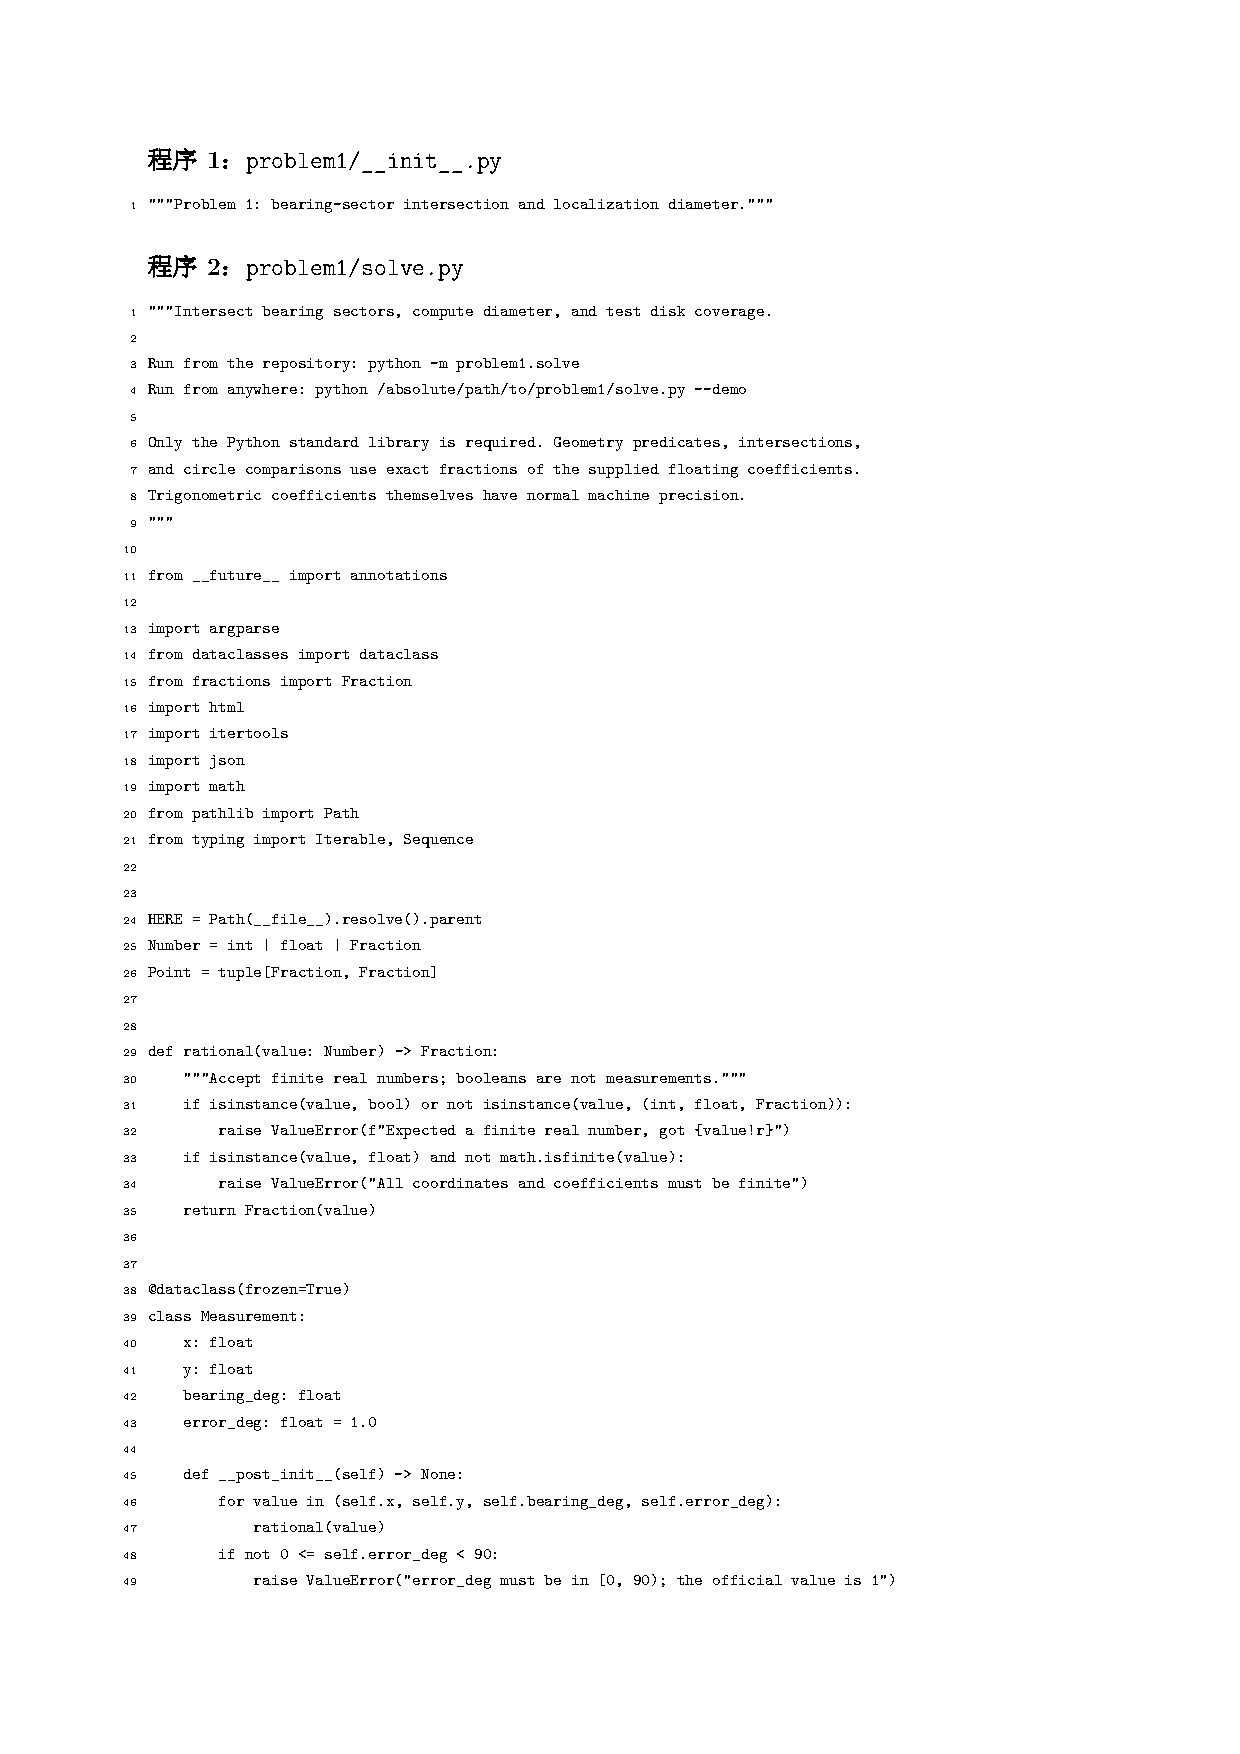
\includepdf[pages=-,pagecommand={\thispagestyle{plain}},fitpaper=false]{code_appendix.pdf}
\end{document}
